\documentclass[12pt]{report}

\usepackage{amsmath, amsfonts, amssymb, amsthm}
\usepackage[normalem]{ulem} % underline (don't redefine emph to underline!)
\usepackage{float} % H float specifier
\usepackage{tabularx} % tabular with column specifier X to break lines
% \usepackage{hyphenat} % disable/enable hyphenation
\usepackage{bookmark} % this loads hyperref
\usepackage{multirow}
\usepackage{booktabs} % (top|mid|bottom)rule and other table stuff
\usepackage{fancyhdr} % fancy headers
\usepackage{systeme} % systems of equation
\usepackage[utf8]{inputenc} % necessary for proper unicode support
\usepackage{parcolumns} % multiple column parallel typesetting
\usepackage[english]{babel} % uncomment this for Angelsächsisch
\usepackage{graphicx} % including graphics
\usepackage{sourcecodepro} % best font
\usepackage{listings} % source code listings
\usepackage{caption} % customize captions in floats (rotate, sideways, ...)
\usepackage{lstlangarm} % custom ARM Assembler keyword list
\usepackage[backend=biber, sorting=none]{biblatex} % better citation
\usepackage[a4paper]{geometry} % customize page geometry

\pagestyle{fancy}
\fancyhead[L]{\rightmark}
\fancyhead[R]{\thepage}
\fancyfoot{}

% non-italic bibliography titles
\DeclareFieldFormat{title}{``#1''}
\DeclareFieldFormat{citetitle}{``#1''}

% umlauts in lstlistings env
\lstset{
    literate={ö}{{\"o}}1
    {ä}{{\"a}}1
    {ü}{{\"u}}1
    {Ö}{{\"O}}1
    {Ä}{{\"A}}1
    {Ü}{{\"U}}1
}

\lstset{
    basicstyle=\scriptsize\ttfamily,
    breaklines=true
}

\lstset {
    frame=single,
    numbers=left,
    stepnumber=1,
    firstnumber=1,
    numberfirstline=true,
    texcl=false
}

\providecommand{\lxor}{\veebar}
\renewcommand{\proofname}{Beweis.}
\newcommand{\sref}[1]{\textsuperscript{\ref{#1}}}
\newcommand{\F}[1]{\mathbb{F}_2^{#1}}

\addbibresource{refs.bib}

\title{
    \textbf{Efficient Implementation Strategies for Block Ciphers on ARMv8}\\
    {\footnotesize Bachelorarbeit}
}
\author{Bastian Engel}
\date{\today}

\begin{document}

\maketitle

\chapter*{Abstract}

Lorem ipsum dolor sit amet, consectetur adipisicing elit, sed do eiusmod tempor
incididunt ut labore et dolore magna aliqua. Ut enim ad minim veniam, quis
nostrud exercitation ullamco laboris nisi ut aliquip ex ea commodo consequat.
Duis aute irure dolor in reprehenderit in voluptate velit esse cillum dolore eu
fugiat nulla pariatur. Excepteur sint occaecat cupidatat non proident, sunt in
culpa qui officia deserunt mollit anim id est laborum.

\chapter*{Declaration}

I hereby declare that ...


\tableofcontents

\chapter{Introduction}
\section{Notation}

\section{Block ciphers}

Securing communication channels between different parties has been a long-term
subject of study for cryptographers and engineers which is essential to our
modern world to cope with ever-increasing amounts of devices producing and
sharing data. The main way to facilitate high-throughput, confidential
communications nowadays is through the use of symmetric cryptography in which
two parties share a common secret, called a key, which allows them to encrypt,
share and subsequently decrypt messages to achieve confidentiality against
third parties. Ciphers can be divided into two categories; block ciphers, which
always encrypt fixed-sized messages called blocks, and stream ciphers, which
continuously provide encryption for an arbitrarily long, constant stream of
data.

A block cipher can be defined as a bijection between the input block (the
message) and the output block (the ciphertext). For any block cipher with block
size $n$, we denote the key-dependent encryption and decryption functions as
$E_K,D_K:\F{n}\rightarrow \F{n}$. The simplest way to
characterize this bijection is through a lookup table which yields the highest
possible performance as each block can be encrypted by one simple lookup
depending on the key and the message. This is not practical though due to most
ciphers working with block and key sizes $n,|K|\geq 64$. For a block cipher
with $n=64,|K|=128$, a space of $2^{64}2^{128}64=2^{198}$ is necessary.
Considering modern consumer hard disks being able to store data in the order of
$2^{40}$, it is easy to see that a lookup table is wholly impractical. We
therefore describe block ciphers algorithmically which opens up possibilities
for different tradeoffs and security concerns.


\subsection{GIFT}

\texttt{GIFT}\cite{gift:2017}, first presented in the \textit{CHES 2017}
cryptographic hardware and embedded systems conference, is a lightweight block
cipher based on a previous design called \texttt{PRESENT}, developed in 2007. Its
goal is to offer maximum security while being extremely light on resources.
Modern battery-powered devices like RFID tags or low-latency operations like
on-the-fly disc encryption present strong hardware and power constraints. GIFT
aims to be a simple, low-energy cipher suited for these kinds of applications.

\texttt{GIFT} comes in two variants; \verb|GIFT-64| working with 64-bit blocks
and GIFT-128 working with 128-bit blocks. In both cases, the key is 128
bits long. The design is a very simple, round-based substitution-permutation
network (SPN). One round consists in a sequential application of the confusion
layer by means of 4-bit S-boxes and subsequent diffusion through bit
permutation. After the bit permutation, a round key is added to the cipher
state and the single round is complete. GIFT-64 uses 28 rounds while
GIFT-128 uses 40 rounds.

\begin{figure}[h!]
    \centering
    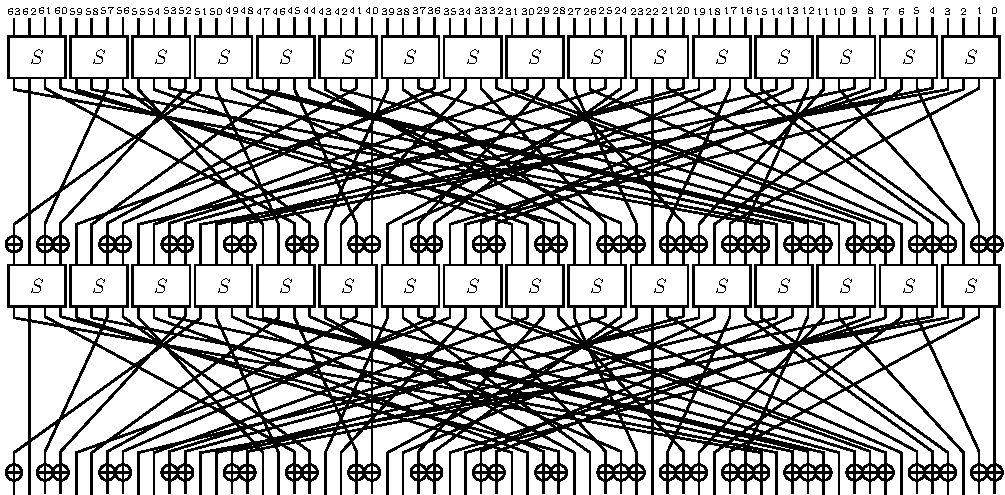
\includegraphics[width=\textwidth]{Figures/GIFT-64.pdf}
    \caption{Two rounds of GIFT-64}
\end{figure}

\subsubsection{Substitution layer}

The input of \texttt{GIFT} is split into 4-bit nibbles which are then fed into
16 S-boxes for GIFT-64 and 32 S-boxes for GIFT-128. The S-box
$S:\F{4}\rightarrow \F{4}$ is defined as follows:

\[
    \begin{array}{l|cccccccccccccccc}
        x & 0 & 1 & 2 & 3 & 4 & 5 & 6 & 7 & 8 & 9 & a & b & c & d & e & f \\
        \hline
        S(x) & 1 & a & 4 & c & 6 & f & 3 & 9 & 2 & d & b & 7 & 5 & 0 & 8 & e
    \end{array}
\]

\subsubsection{Permutation layer}

The permutation $P$ works on individual bits and maps bit $b_i$ to $b_{P(i)}$.
The different permutations for GIFT-64 and GIFT-128 can be expressed by:

\begin{align*}
    P_{64}(i)&=4\left\lfloor\frac{i}{16}\right\rfloor+16\left(\left(3\left\lfloor\frac{i\bmod 16}{4}\right\rfloor+(i\bmod 4)\right)\bmod 4\right)+(i\bmod 4) \\
    P_{128}(i)&=4\left\lfloor\frac{i}{16}\right\rfloor+32\left(\left(3\left\lfloor\frac{i\bmod 16}{4}\right\rfloor+(i\bmod 4)\right)\bmod 4\right)+(i\bmod 4) \\
\end{align*}

\subsubsection{Round key addition}

The last step of each round consists in XORing a round key $R_{i}$ to the cipher
state. The new cipher state $x_{i+1}$ after each full round is therefore given
by

\[
    x_{i+1}=P(S(x_i))\oplus R_i
\]

\subsubsection{Round key extraction and key schedule}

Round key extraction differs for GIFT-64 and GIFT-128. Let
$K_{(128)}=k_7||k_6||\dots||k_0$ denote the 128-bit key state.

\paragraph{GIFT-64}. We extract two words $U_{(16)}||V_{(16)}=k_1||k_0$ from the key
state. These are then added to round key $R_{(64)}$: $R_{4i+1}\leftarrow
U_i,R_{4i}\leftarrow V_i$.

\paragraph{GIFT-128}. We extract two words
$U_{(32)}||V_{(32)}=k_5||k_4||k_1||k_0$ from the key state. These are then
added to round key $R_{(128)}$: $R_{4i+2}\leftarrow U_i,R_{4i+1}\leftarrow
V_i$.

In both cases, we additionally XOR a round constant $C_{(6)}$ to bit positions
$n-1,23,19,15,11,7,3$. The round constants are generated using a 6-bit affine
linear-feedback shift register and have the following values:\\

\begin{tabular}{r|l}
    \textbf{Rounds} & \textbf{Constants} \\
    \hline
    \textbf{1 - 16} &  \small\texttt{01,03,07,0F,1F,3E,3D,3B,37,2F,1E,3C,39,33,27,0E} \\
    \textbf{17 - 32} & \small\texttt{1D,3A,35,2B,16,2C,18,30,21,02,05,0B,17,2E,1C,38} \\
    \textbf{33 - 48} & \small\texttt{31,23,06,0D,1B,36,2D,1A,34,29,12,24,08,11,22,04}
\end{tabular}\\

The key state is then updated by individually rotating $k_1$ and $k_0$ and
rotating the new state $32$ bits to the right:

\[
    k_7||k_6||\dots||k_1||k_0\leftarrow k_1\ggg 2||k_0\ggg 12||k_7||k_6||\dots||k_3||k_2
\]

\subsection{Camellia}

Camellia\cite{camellia:2001} is a block cipher jointly developed by NTT and
Mitsubishi Electric Corporation and first published in 2001. Following AES
specifications, it is able to encrypt 128-bit blocks using either 128-, 196- or
256-bit keys and claims to possess similar performance and security levels as
the AES finalists.

\subsubsection{Encryption overview}

The encryption process has an 18-round Feistel structure for 128-bit keys and a
24-round Feistel structure for 192/256-bit key and employs key whitening to
increase security. First, subkeys $kw_{t(64)}(t=0,1,2,3)$,
$k_{u(64)}(u=0,1,\dots,(17|23)$ and $kl_{v(64)}(v=0,1,2,3)$ are generated from
the master key. Then, pre-whitening keys are applied to the plaintext
$m_{(128)}=L_{(64)}||R_{(64)}$:

\[
    (L||R)\leftarrow (L||R)\oplus (kw_0||kw_1)
\]

The next steps differ for 128-bit and 192/256-bit keys in the number of rounds:

\begin{table}[h!]
    \centering
    \caption{Camellia encryption}
    \begin{tabular}{lll}
        \toprule
        Round $r$ & 128-bit keys & 192/256-bit keys \\
        \midrule
        0-4 & $(L||R)\leftarrow FE(L,R,k_r)$ & $(L||R)\leftarrow FE(L,R,k_r)$ \\
        \midrule
        5 & {$\!\begin{aligned}&(L||R)\leftarrow FE(L,R)\\&(L||R)\leftarrow FLL(L,R,kl_0,kl_1)\end{aligned}$} & {$\!\begin{aligned}&(L||R)\leftarrow FE(L,R)\\&(L||R)\leftarrow FLL(L,R,kl_0,kl_1)\end{aligned}$} \\
        \midrule
        6-10 & $(L||R)\leftarrow FE(L,R,k_r)$ & $(L||R)\leftarrow FE(L,R,k_r)$ \\
        \midrule
        11 & {$\!\begin{aligned}&(L||R)\leftarrow FE(L,R)\\&(L||R)\leftarrow FLL(L,R,kl_2,kl_3)\end{aligned}$} & {$\!\begin{aligned}&(L||R)\leftarrow FE(L,R)\\&(L||R)\leftarrow FLL(L,R,kl_2,kl_3)\end{aligned}$} \\
        \midrule
        12-16 & $(L||R)\leftarrow FE(L,R,k_r)$ & $(L||R)\leftarrow FE(L,R,k_r)$ \\
        \midrule
        17 & & {$\!\begin{aligned}&(L||R)\leftarrow FE(L,R)\\&(L||R)\leftarrow FLL(L,R,kl_4,kl_5)\end{aligned}$} \\
        \midrule
        18-23 & & $(L||R)\leftarrow FE(L,R,k_r)$ \\
        \bottomrule
    \end{tabular}
\end{table}

Finally, $R$ and $L$ are concatenated and XORed with the post-whitening keys to
obtain the cipher text $c_{(128)}$:

\[
    c=(R||L)\oplus (kw_2)||kw_3)
\]

\subsubsection{Components}

We will give an overview of the main functional components of Camellia.

\paragraph{Feistel round function $FE$:}

\begin{align*}
    FE:(\F{64})^3 &\rightarrow (\F{64})^2 \\
    (L_{(64)},R_{(64)},k_{(64)})&\mapsto (R\oplus F(L,k), L)
\end{align*}

\paragraph{SP-function $F$:}

\begin{align*}
    F:(\F{64})^2 &\rightarrow \F{64} \\
    (X_{(64)},k_{(64)})&\mapsto P(S(X\oplus k))
\end{align*}

\paragraph{Substitution function $S$:}

\begin{align*}
    S:\F{64} &\rightarrow \F{64} \\
    \begin{aligned}
        l_{0(8)}||l_{1(8)}||l_{2(8)}||l_{3(8)}&||\\
        l_{4(8)}||l_{5(8)}||l_{6(8)}||l_{7(8)}&
    \end{aligned}&\mapsto
    \begin{aligned}
        s_0(l_0)||s_1(l_1)||s_2(l_2)||s_3(l_3)&||\\
        s_1(l_4)||s_2(l_5)||s_3(l_6)||s_0(l_7)&
    \end{aligned},
\end{align*}

with 8-bit S-boxes $s_0,s_1,s_2,s_3:\F{8}\rightarrow \F{8}$.

\paragraph{Permutation function $P$:}

\begin{align*}
    P:\F{64} &\rightarrow \F{64} \\
    \begin{pmatrix}z_7\\z_6\\z_5\\z_4\\z_3\\z_2\\z_1\\z_0\end{pmatrix}&\mapsto
    \begin{pmatrix}
        0 & 1 & 1 & 1 & 1 & 0 & 0 & 1 \\
        1 & 0 & 1 & 1 & 1 & 1 & 0 & 0 \\
        1 & 1 & 0 & 1 & 0 & 1 & 1 & 0 \\
        1 & 1 & 1 & 0 & 0 & 0 & 1 & 1 \\
        0 & 1 & 1 & 1 & 1 & 1 & 1 & 0 \\
        1 & 0 & 1 & 1 & 0 & 1 & 1 & 1 \\
        1 & 1 & 0 & 1 & 1 & 0 & 1 & 1 \\
        1 & 1 & 1 & 0 & 1 & 1 & 0 & 1
    \end{pmatrix}\begin{pmatrix}z_7\\z_6\\z_5\\z_4\\z_3\\z_2\\z_1\\z_0\end{pmatrix}
\end{align*}

\paragraph{$FL$ layer function $FLL$:}

\begin{align*}
    FLL:(\F{64})^4 &\rightarrow (\F{64})^2 \\
    (X_{L(64)},X_{R(64)},k_{0(64)},k_{1(64)})&\mapsto (FL(X_L,k_0),FL^{-1}(X_R,k_1))
\end{align*}

\paragraph{$FL$:}

\begin{align*}
    FL:(\F{64})^2 &\rightarrow \F{64} \\
    (X_{L(32)}||X_{R(32)},k_{L(32)}||k_{R(32)})&\mapsto (Y_{L(32)}||Y_{R(32)}),
\end{align*}

where

\begin{align*}
    Y_{R(32)}&=((X_L\cap k_{L})\lll_1)\oplus X_{R} \\
    Y_{L(32)}&=(Y_R\cup k_{R})\oplus X_{L}
\end{align*}

\paragraph{$FL^{-1}$:}

\begin{align*}
    FL^{-1}:(\F{64})^2 &\rightarrow \F{64} \\
    (Y_{L(32)}||Y_{R(32)},k_{L(32)}||k_{R(32)})&\mapsto (X_{L(32)}||X_{R(32)}),
\end{align*}

where

\begin{align*}
    X_{L(32)}&=(Y_R\cup k_{R})\oplus Y_{L} \\
    X_{R(32)}&=((X_L\cap k_{L})\lll_1)\oplus Y_{R}
\end{align*}

\section{The ARMv8 platform}

With small devices and embedded processors becoming ever more ubiquitous and
essential in areas like consumer electronics or industrial and IoT
applications, the need for low-power, high-performance microprocessors has
increased steadily. With more than 250 billion chips shipped, semiconductors
designed by ARM power 95\% of mobile devices and have found a great many
applications due to their high performance and low power
consumption\cite{armcompany}. The ODROID-N2+\cite{odroidn2} development board
we are using is based on the big.LITTLE architecture and is powered by a
quad-core ARM Cortex-A73 processor and a weaker dual-core ARM Cortex-A53 for
power efficiency. Both these processors are part of the eight generation of ARM
designs known as ARMv8\cite{armv8:2013}.

ARMv8 defines three architecture profiles for different use cases as well as
dynamic execution states with corresponding instruction sets. This work will
focus on the A profile running in the AArch64 state utilizing the A64
instruction set with NEON and crypto extensions.

\begin{table}[h!]
    \centering
    \caption{ARMv8 profiles}
    \begin{tabularx}{\textwidth}{lX}
        \toprule
        Profile & Description \\
        \midrule
        Application (A) & Traditional use with virtual memory and privilege level support \\
        Real-time (R) & Real-time, low-latency, deterministic embedded systems \\
        Microcontroller (M) & Very low-power, fast-interrupt embedded systems \\
        \bottomrule
    \end{tabularx}
\end{table}

\begin{table}[h!]
    \centering
    \caption{ARMv8 execution states}
    \begin{tabularx}{\textwidth}{llX}
        \toprule
        Execution state & Usage & Instruction sets \\
        \midrule
        AArch32 & 32-bit compatibility & A32/T32 \\
        AArch64 & 64-bit & A64 \\
        \bottomrule
    \end{tabularx}
\end{table}

\subsection{General architecture}

ARMv8 is a RISC architecture employing simple data processing instructions
operating only on registers as well as dedicated load/store instructions to
transfer data from register to memory and back. This enables faster execution
of individual instructions, a simplier pipeline design, predictable instruction
timings and fewer addressing modes.

The A64 instruction set defines 31 64-bit general-purpose registers
\texttt{X0-X30} which can also be accessed as 32-bit registers \texttt{W0-W30}.
Values are loaded from and stored to memory using \texttt{LDR}/\texttt{STR}.
Data processing instructions generally use explicit output registers instead of
overwriting the first input register.

\begin{table}[h!]
    \centering
    \small
    \caption{A64 addressing modes}
    \begin{tabularx}{\textwidth}{llX}
        \toprule
        Addressing mode & Example & Description \\
        \midrule
        Base register & \texttt{LDR W0, [X1]} & \texttt{W0 = *(X1);} \\
        Offset & \texttt{LDR W0, [X1, \#12]} & \texttt{W0 = *(X1 + 12);} \\
        Pre-indexing & \texttt{LDR W0, [X1, \#12]!} & \texttt{X1 += 12; W0 = *(X1);} \\
        Post-indexing & \texttt{LDR W0, [X1], \#12} & \texttt{W0 = *(X1); X1 += 12;} \\
        \bottomrule
    \end{tabularx}
\end{table}

\subsection{NEON}
\label{ss:neon}

ARMv8 supports single-instruction, multiple-data (SIMD) processing. These systems
allow the programmer to store multiple pieces of data in a vector and work on
them in parallel to speed up calculations. The A64 instruction set defines two
possible SIMD implementations:

\begin{enumerate}
    \item Advanced SIMD, known as NEON
    \item Scalable Vector Extension (SVE)
\end{enumerate}

We will take a look at NEON as this is the type of vector processing supported
by the Cortex-A73 processor.

The register file of the NEON unit is made up of 32 quad-word (128-bit)
registers \texttt{V0-V31}, each extending the standard 64-bit floating-point
registers \mbox{\texttt{D0-31}}. These registers are divided into equally sized
lanes on which vector instructions operate. Figure \ref{fig:regdivs} shows
valid ways to interpret the register \texttt{V0}.

\begin{figure}[h!]
    \centering
    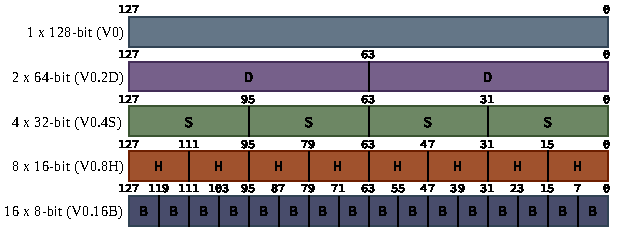
\includegraphics[width=\textwidth]{Figures/V_register.pdf}
    \caption{Divisions of the V0 register}
    \label{fig:regdivs}
\end{figure}

NEON instructions interpret their operands' layouts (i.e. lane count and width)
through the use of suffixes such as \texttt{.4S} or \texttt{.8H}. Adding eight
16-bit halfwords stored in \texttt{V1} and \texttt{V2} can be done as follows:

\begin{center}
    \texttt{ADD V0.8H, V1.8H, V2.8H}
\end{center}

\begin{figure}[h!]
    \centering
    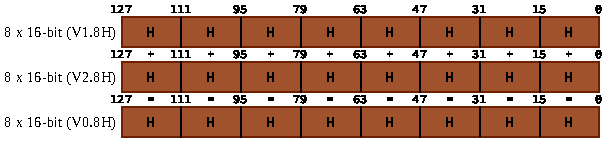
\includegraphics[width=\textwidth]{Figures/vector_add.pdf}
    \caption{Addition of two vector registers}
\end{figure}

\subsection{NEON Intrinsics}

The header file \texttt{<arm\_neon.h>} provides ARM-specific data and function
definitions including vector data types and C functions for working with these
vectors. These functions are known as NEON intrinsics \cite{neonintr:2022} and
give the programmer a high-level interface to most NEON instructions. Major
advantages of this approach include the ease of development as the compiler
takes over register allocation and load/store operations as well as performance
benefits through compiler optimizations.

Standard vector data types have the format \texttt{uintnxm\_t} with lane width
$n$ in bits and and lane count $m$. Array types of the format
\texttt{uintnxmxc\_t}, $c\in\{2,3,4\}$ are also defined which are used in
operations requiring multiple parameters like \texttt{TBL} or pairwise
load/stores. Intrinsics include the operation name and lane data format as well
as an optional \texttt{q} suffix to indicate operation on a 128-bit register.
Multiplying eight pairs of 16-bit numbers \texttt{a,b} for example can be done
via the following:

\begin{center}
    \texttt{uint16x8\_t result = vmulq\_u16(a, b);}
\end{center}

In this case, the compiler allocates vector registers for \texttt{a},
\texttt{b} and \texttt{result} and assembles the intrinsic to \texttt{MUL
Vr.8H, Va.8H, Vb.8H}. Necessary loads and stores for the result and parameters
are also handled automatically. Of special interest to us are the following
intrinsics, each existing in different variants with different lane widths and
also array types: \\

\begin{table}[h!]
    \centering
    \footnotesize
    \caption{Common NEON intrinsics}
    \begin{tabularx}{\textwidth}{llX}
        \toprule
        Intrinsic && Summary \\
        \midrule
        \texttt{uint64\_t} & \texttt{vgetq\_lane\_u64(void)} & Extract a single lane \\
        \midrule
        \texttt{void} & \texttt{vsetq\_lane\_u64(uint64\_t)} & Insert a single lane \\
        \midrule
        \texttt{uint64x2\_t} & \texttt{vdupq\_n\_u64(uint64\_t)} & Initialize all lanes to same value \\
        \midrule
        \texttt{void} & \texttt{vst1q\_u64(uint64\_t*, uint64x2\_t)} & Store from register to memory \\
        \midrule
        \texttt{uint64x2\_t} & \texttt{vld1q\_u64(uint64\_t*, uint64x2\_t)} & Load from memory to register \\
        \midrule
        \texttt{uint8x16\_t} & \texttt{veorq\_u8(uint8x16\_t, uint8x16\_t)} & bitwise XOR \\
        \midrule
        \texttt{uint8x16\_t} & \texttt{vandq\_u8(uint8x16\_t, uint8x16\_t)} & bitwise AND \\
        \midrule
        \texttt{uint8x16\_t} & \texttt{vorrq\_u8(uint8x16\_t, uint8x16\_t)} & bitwise OR \\
        \midrule
        \texttt{uint8x16\_t} & \texttt{vmvnq\_u8(uint8x16\_t)} & bitwise NOT \\
        \midrule
        \texttt{uint8x16\_t} & \texttt{vqtbl2q\_u8(uint8x16\_t, uint8x16\_t)} & permutation (\texttt{TBL}) \\
        \bottomrule
    \end{tabularx}
\end{table}

\chapter{Implementation strategies}

Due to the structural differences of SPN- and Feistel network-based ciphers, we
shall analyze these two separately.

\section{Strategies for \texttt{GIFT}}

Three implementation strategies for substitution-permutation networks are
introduced by \cite{implx86:2014}:

\begin{itemize}
    \item Table-based implementations
    \item \texttt{vperm} implementations
    \item Bitslice implementations
\end{itemize}

\subsection{Table-based}

Table-driven programming is a simple way to increase performance of operations
by tabulating the results, therefore requiring only a single memory access to
acquire the result. This approach is obviously limited to manageable table
sizes, so while tabulating a function like the AES S-box
$S_{AES}:\F{8}\rightarrow \F{8}$ requires only $2^{11}$ space,
tabulating the \texttt{GIFT} permutation layer
$P_{GIFT}:\F{64}\rightarrow \F{64}$ would require
$2^{70}$ space, which is totally unfeasible.

A common approach is to tabulate the output of each S-box, including the
diffusion layer, and then XORing the results together. Let $n$ denote the
internal cipher state size and $s$ the size of a single S-box in bits. For each
S-box $S_i,i\in\{0,\dots,\frac{n}{s}\}$, we can construct a mapping
$T_i:\F{s}\rightarrow \F{n}$ representing substitution with subsequent
permutation of that single S-box. The cipher state before round key addition is
then given by $\bigoplus_{i=0}^{\frac{n}{s}-1}{T_i(m_i)}$ for each $s$-bit
message chunk $m_i$. This approach requires space of
$\frac{n}{s}|\F{s}|n=\frac{n^2 2^s}{s}$ bits, which, for \texttt{GIFT-64},
results in a manageable size of $\frac{64^2 2^4}{4}=2^{14}$ bits which equals
$16$ KiB.

\subsubsection{Constructing the tables}

For \texttt{GIFT-64}, table construction is relatively straightforward and can
be done as follows:

\begin{lstlisting}[caption={Table construction algorithm}, label={lst:tables}, escapechar=|]
    tables <- [][]
    for sbox_index from 0 to 15 do
        for sbox_input from 0 to 15 do|\label{lst:tablesbox}|
            output <- sbox(sbox_input)
            output <- permute(output << (4 * sbox_index))
            tables[sbox_index][sbox_input] <- output
\end{lstlisting}

Implementing this algorithm gives us the following table representing the first
and second S-box.

\[
    \begin{array}{l|l|l|c}
        x & T_0(x) & T_1(x) & \dots \\
        \hline
        0x0 & 0x1               & 0x1000000000000   & \dots \\
        0x1 & 0x8000000020000   & 0x800000002       & \dots \\
        0x2 & 0x400000000       & 0x40000           & \dots \\
        0x3 & 0x8000400000000   & 0x800040000       & \dots \\
        0x4 & 0x400020000       & 0x40002           & \dots \\
        0x5 & 0x8000400020001   & 0x1000800040002   & \dots \\
        0x6 & 0x20001           & 0x1000000000002   & \dots \\
        0x7 & 0x8000000000001   & 0x1000800000000   & \dots \\
        0x8 & 0x20000           & 0x2               & \dots \\
        0x9 & 0x8000400000001   & 0x1000800040000   & \dots \\
        0xa & 0x8000000020001   & 0x1000800000002   & \dots \\
        0xb & 0x400020001       & 0x1000000040002   & \dots \\
        0xc & 0x400000001       & 0x1000000040000   & \dots \\
        0xd & 0x0               & 0x0               & \dots \\
        0xe & 0x8000000000000   & 0x800000000       & \dots \\
        0xf & 0x8000400020000   & 0x800040002       & \dots
    \end{array}
\]

The tables for \texttt{GIFT-128} can be generated in a similar way by looping
through all 32 S-boxes instead of 16 on line \ref{lst:tablesbox}.

\subsection{Using \texttt{vperm}}

The plenitude of different processing instructions introduced by
NEON\ref{ss:neon} allow flexible ways to further speed up algorithms having
reached their optimizational limit on non-SIMD platforms. \texttt{vperm}, a
general term standing for \textit{vector permute}, is a common instruction on
SIMD machines. Called \texttt{TBL} on NEON, it is used for parallel table
lookups and arbitrary permutations. It takes two inputs to perform a lanewise
lookup:

\begin{enumerate}
    \item A register with lookup values
    \item One or more registers containing data
\end{enumerate}

\subsubsection{S-box lookup}

This instruction can be used to implement S-box lookup of all 16 S-boxes in a
single instruction. We do this by packing our 64-bit cipher state
$s=s_{15}||s_{14}||\dots||s_0$ into a vector register $V_0$. Because we can
only operate on whole bytes, we put each 4-bit S-box into an 8-bit lane which
neatly fits into the 128-bit registers. We then put the S-box itself into
register $V_1$ which will be used as the data register for the table lookup.

The confusion layer can now be performed through one \texttt{TBL} instruction:

\begin{center}
    \texttt{TBL V0.16B, V1.16B, V0.16B}
\end{center}

\begin{figure}[h!]
    \centering
    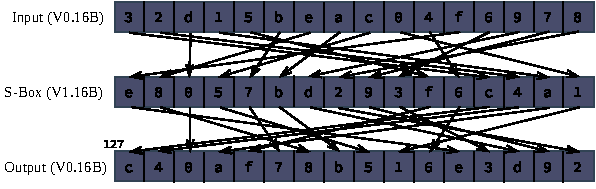
\includegraphics[width=\textwidth]{Figures/tbl_example.pdf}
    \caption{Performing the S-Box lookup in parallel}
\end{figure}

\subsection{Bitslicing}

Bitsliced implementation techniques were first introduced to improve the performance
of DES in 1997 and work by viewing a processor with $n$-bit registers as a
machine capable of executing $n$ bitwise operations at
once\cite{desslicing:1997}. Bitslicing offers a performance advantage by
splitting up $n$ bits into $m$ slices to achieve a more efficient
representation which can exploit this bitwise parallelism. The structure of
\texttt{GIFT} naturally offers possibilities for bitslicing. We split the
cipher state bits $b_{63}b_{62}\dots b_0$ into four slices $S_i,
i\in\{0,1,2,3\}$ such that the $i$-th slice contains all $i$-th bits of the
individual S-boxes. This is equivalent to transposing the bit matrix.

\[
    S=\begin{bmatrix}
        S_0\\
        S_1\\
        S_2\\
        S_3
    \end{bmatrix}
    =\begin{bmatrix}
        b_{60}b_{56}b_{52}\dots b_0\\
        b_{61}b_{57}b_{53}\dots b_1\\
        b_{62}b_{58}b_{54}\dots b_2\\
        b_{63}b_{59}b_{55}\dots b_3
    \end{bmatrix}
\]

\subsubsection{Parallel S-Boxes}

This representation offers multiple advantages. We first note that computation
of the S-box can be executed in parallel, similar to the \texttt{vperm}
technique above. This can be done by finding a bitwise instruction sequence to
apply the S-box which has already been proposed by the original \texttt{GIFT}
authors:

\begin{align*}
    S_1&\leftarrow S_1\oplus (S_0\land S_2) \\
    t&\leftarrow S_0\oplus (S_1\land S_3) \\
    S_2&\leftarrow S_2\oplus (t\lor S_1) \\
    S_0&\leftarrow S_3\oplus S_2 \\
    S_1&\leftarrow S_1\oplus S_0 \\
    S_0&\leftarrow \lnot S_0 \\
    S_2&\leftarrow S_2\oplus (t\land S_1) \\
    S_3&\leftarrow t
\end{align*}

This is very efficient as it only requires six XOR-, three AND and one OR
operation.

An important property of the permutation is the fact that bits always stay in
their slice. This means we can decompose the permutation $P$ into four
permutations $P_i,i\in\{0,1,2,3\}$ and apply these permutations
separately to each slice. One possible way to implement a permutation $P_i$ in
software is to mask off all bits individually, shift them to their correct
position and OR them together:

\[
    P_i(S_i)=\bigvee_{k=0}^{15}{(S_i\land m_i) \ll s_i}
\]

This approach requires $47$ operations, meaning all four permutations require
over $150$ operations which would present a major bottleneck to the round
function. We can improve on this by working on multiple message blocks at once
and using the aforementioned \texttt{vperm} instruction to implement the bit
shuffling. We then need only four instructions for the complete diffusion
layer.

\subsubsection{Using \texttt{vperm} for slice permutation}

We cannot use the \texttt{TBL} instruction directly as we need to shuffle
individual bits, but the smallest data we can operate on are bytes. We
therefore encrypt $8n$ messages at once which allows us to create bytewise
groupings. These messages are put into $4m$ registers with register $R_{4i}$
containing $S_0$, register $R_{4i+1}$ containing $S_1$ and so forth. With block
size $BS$ and register size $RS$, the following must hold:

\[
    8n\cdot BS=4m\cdot RS
\]

In the case of \texttt{GIFT-64} with $BS=64$ and ARM NEON with $RS=128$, we get

\[
    8n\cdot 64=4m\cdot 128\Leftrightarrow n=m
\]

$n=m=1$ would be a valid choice which yields eight messages divided into four
registers. We choose $n=m=2$ so we can directly utilize the algorithm for bit
packing presented by the original GIFT authors, although it is simple to adapt
this algorithm to only four registers and eight messages by adjusting the
\texttt{SWAPMOVE} shift and mask values.

\subsubsection{Packing the data into bitslice format}

Let $a,b,\dots,p$ be sixteen messages of length $64$ with subscripts denoting
individual bits. We first put these messages into eight SIMD registers
$V_0,V_1,\dots,V_7$:

\begin{alignat*}{3}
    V_0&=b||a\qquad V_4&&=j||&&i \\
    V_1&=d||c\qquad V_5&&=l||&&k \\
    V_2&=f||e\qquad V_6&&=n||&&m \\
    V_3&=h||g\qquad V_7&&=p||&&o
\end{alignat*}

We then use the \texttt{SWAPMOVE} technique to bring the data into bitslice
format. This operation operates on two registers $A,B$ using mask $M$ and shift
value $N$. It swaps bits in $A$ masked by $(M\ll N)$ with bits in $B$ masked by
$M$ in using only three XOR-, one AND- and two shift operations.

\begin{align*}
    &\text{SWAPMOVE}(A,B,M,N): \\
    &\qquad T=((A\gg N)\oplus B)\land M \\
    &\qquad B=B\oplus T \\
    &\qquad A=A\oplus (T\ll N) \\
\end{align*}

One caveat of this approach is the fact that NEON registers cannot be shifted
in their entirety due to the fact bits are not able to cross lanes. This leads
to the problem of being able to shift at most two lanes of 64 bits at once. We
thus need to implement the \texttt{shr(V,n)} and \texttt{shl(V,n)} operations
on our own. This can be done by first extracting the 64-bit lanes $a,b$ out of
$V=b||a$, shifting the lanes individually and finally shifting and ORing the
crossing bits back into the other lane.

\begin{alignat*}{2}
    &\text{shl}(V,n): \\
    &\qquad a,b&&=V[0],V[1] \\
    &\qquad c&&=(a\gg (64-n)) \\
    &\qquad V[0]&&=(a\ll n) \\
    &\qquad V[1]&&=(b\ll n)\lor c
\end{alignat*}

The following operations group all $i$-th bits of the messages $a,c,\dots,o$
into bytes and puts these into the lower half of the registers $V_{i\bmod 8}$.
The same is done for messages $b,d,\dots,p$, only differing in that the bytes
are put into the upper half of the registers.

\begin{align*}
    &\text{SWAPMOVE}(V_0,V_1,0x5555\dots 55,1) &\text{SWAPMOVE}(V_4,V_5,0x5555\dots 55,1) \\
    &\text{SWAPMOVE}(V_2,V_3,0x5555\dots 55,1) &\text{SWAPMOVE}(V_6,V_7,0x5555\dots 55,1) \\
    &\text{SWAPMOVE}(V_0,V_2,0x3333\dots 33,2) &\text{SWAPMOVE}(V_4,V_6,0x3333\dots 33,2) \\
    &\text{SWAPMOVE}(V_1,V_3,0x3333\dots 33,2) &\text{SWAPMOVE}(V_5,V_7,0x3333\dots 33,2) \\
    &\text{SWAPMOVE}(V_0,V_4,0x0f0f\dots 0f,4) &\text{SWAPMOVE}(V_1,V_5,0x0f0f\dots 0f,4) \\
    &\text{SWAPMOVE}(V_2,V_6,0x0f0f\dots 0f,4) &\text{SWAPMOVE}(V_3,V_7,0x0f0f\dots 0f,4) \\
\end{align*}

With $Ax=o_xm_xk_xj_xg_xe_xc_xa_x$ and $Bx=p_xn_xl_xi_xh_xf_xd_xb_x$ denoting
byte groups, our data now has the following permutation-friendly format:

\scriptsize
\[
    \begin{array}{c|llllllll|llllllll}
        n & 15 & 14 & 13 & 12 & 11 & 10 & 9 & 8 & 7 & 6 & 5 & 4 & 3 & 2 & 1 & 0 \\
        \hline
        V_0 & B56 & B48 & B40 & B32 & B24 & B16 & B8  & B0 & A56 & A48 & A40 & A32 & A24 & A16 & A8  & A0 \\
        V_1 & B57 & B49 & B41 & B33 & B25 & B17 & B9  & B1 & A57 & A49 & A41 & A33 & A25 & A17 & A9  & A1 \\
        V_2 & B58 & B50 & B42 & B34 & B26 & B18 & B10 & B2 & A58 & A50 & A42 & A34 & A26 & A18 & A10 & A2 \\
        V_3 & B59 & B51 & B43 & B35 & B27 & B19 & B11 & B3 & A59 & A51 & A43 & A35 & A27 & A19 & A11 & A3 \\
        V_4 & B60 & B52 & B44 & B36 & B28 & B20 & B12 & B4 & A60 & A52 & A44 & A36 & A28 & A20 & A12 & A4 \\
        V_5 & B61 & B53 & B45 & B37 & B29 & B21 & B13 & B5 & A61 & A53 & A45 & A37 & A29 & A21 & A13 & A5 \\
        V_6 & B62 & B54 & B46 & B38 & B30 & B22 & B14 & B6 & A62 & A54 & A46 & A38 & A30 & A22 & A14 & A6 \\
        V_7 & B63 & B55 & B47 & B39 & B31 & B23 & B15 & B7 & A63 & A55 & A47 & A39 & A31 & A23 & A15 & A7
    \end{array}
\]
\normalsize

Although this would already work, we prefer to have only bits of the same
messages in each register - otherwise the permutation would need to operate on
two source registers with the added requirement of storing the pre-permutation
values for the first four registers, slowing down the round function through
superfluous load/stores. This transformation is trivial by use of
\texttt{TBL} with two data source operands. The final data format we operate on
is as follows:

\[
    \scriptsize
    \begin{array}{c|llllllll|llllllll}
        n & 15 & 14 & 13 & 12 & 11 & 10 & 9 & 8 & 7 & 6 & 5 & 4 & 3 & 2 & 1 & 0 \\
        \hline
        V_0 & A60 & A56 & A52 & A48 & A44 & A40 & A36 & A32 & A28 & A24 & A20 & A16 & A12 & A8  & A4 & A0 \\
        V_1 & A61 & A57 & A53 & A49 & A45 & A41 & A37 & A33 & A29 & A25 & A21 & A17 & A13 & A9  & A5 & A1 \\
        V_2 & A62 & A58 & A54 & A50 & A46 & A42 & A38 & A34 & A30 & A26 & A22 & A18 & A14 & A10 & A6 & A2 \\
        V_3 & A63 & A59 & A55 & A51 & A47 & A43 & A39 & A35 & A31 & A27 & A23 & A19 & A15 & A11 & A7 & A3 \\
        V_4 & B60 & B56 & B52 & B48 & B44 & B40 & B36 & B32 & B28 & B24 & B20 & B16 & B12 & B8  & B4 & B0 \\
        V_5 & B61 & B57 & B53 & B49 & B45 & B41 & B37 & B33 & B29 & B25 & B21 & B17 & B13 & B9  & B5 & B1 \\
        V_6 & B62 & B58 & B54 & B50 & B46 & B42 & B38 & B34 & B30 & B26 & B22 & B18 & B14 & B10 & B6 & B2 \\
        V_7 & B63 & B59 & B55 & B51 & B47 & B43 & B39 & B35 & B31 & B27 & B23 & B19 & B15 & B11 & B7 & B3
    \end{array}
\]

We can now create permutation tables using the specification of the individual
slice permutations $P_i$ which are then applied to $V_i$ and $V_{i+4}$
respectively:

\[
    \begin{array}{c|llllllllllllllll}
        j & 0 & 1 & 2 & 3 & 4 & 5 & 6 & 7 & 8 & 9 & 10 & 11 & 12 & 13 & 14 & 15 \\
        \hline
        P_0(j) & 0 & 12 & 8 & 4 & 1 & 13 & 9 & 5 & 2 & 14 & 10 & 6 & 3 & 15 & 11 & 7 \\
        P_1(j) & 4 & 0 & 12 & 8 & 5 & 1 & 13 & 9 & 6 & 2 & 14 & 10 & 7 & 3 & 15 & 11 \\
        P_2(j) & 8 & 4 & 0 & 12 & 9 & 5 & 1 & 13 & 10 & 6 & 2 & 14 & 11 & 7 & 3 & 15 \\
        P_3(j) & 12 & 8 & 4 & 0 & 13 & 9 & 5 & 1 & 14 & 10 & 6 & 2 & 15 & 11 & 7 & 3
    \end{array}
\]

One thing to take note of is the original permutation values only show where a
given byte should land, not which byte belongs to a certain position - i.e. for
$P_0$, byte 1 should land in position 12, but the byte belonging to position 1
is byte 4. Because \texttt{TBL} works in the latter way, we have to do some
trivial rearrangements.

Assuming the correct permutation values are put into registers
$V_8,V_9,V_{10},V_{11}$, this now allows us to compute the permutation layer
for all 16 blocks in only eight permutation instructions.

\begin{alignat*}{2}
    &\texttt{TBL V0, V0, V8}\qquad &&\texttt{TBL V1, V1, V9} \\
    &\texttt{TBL V4, V4, V8}\qquad &&\texttt{TBL V5, V5, V9} \\
    &\texttt{TBL V2, V2, V10}\qquad &&\texttt{TBL V3, V3, V11} \\
    &\texttt{TBL V6, V6, V10}\qquad &&\texttt{TBL V7, V7, V11}
\end{alignat*}

\subsubsection{Round key function}

In contrast to packing and unpacking of data which is only done once in the
beginning and end, a round key is derived for every round, so the round key
derivation function needs to be as fast as possible. A simple but naive
approach for one round would be to generate a single round key, copy it 15
times and pack the resulting registers similar to how we proceed with the
messages. Due to the cost of packing the messages, this is prohibitivly
expensive. Because we know where each byte group ends up after packing, we can
directly XOR the round key bits to the correct position. Extending these bits
to bytes can then be done simply by repeatedly shifting and ORing the registers
together.

\section{Strategies for Camellia}

\subsection{Platform-independent techniques}

The original paper proposes various platform-independent ways to implement
Camellia efficiently. Only some of these apply to the ARMv8 architecture since
features like the inline barrel shifter and bitfield manipulation instructions
generally offer better performance.

\begin{description}
    \item[XOR cancellation property in key schedule:]
        While deriving $K_A$ in the key schedule, the instruction sequence

        \begin{align*}
            K_A&\leftarrow K_L\oplus K_R \\
            K_A&\leftarrow FE(FE(K_A, \Sigma_0), \Sigma_1) \\
            K_A&\leftarrow K_A\oplus K_L \\
        \end{align*}

        causes cancellations, allowing us to eliminate some operations by
        replacing it with the following:

        \begin{align*}
            K_{A_L}&\leftarrow F(K_{L_R}\oplus F(K_{L_L}, \Sigma_0)) \\
            K_{A_R}&\leftarrow F(K_{L_L}\oplus \Sigma_1)
        \end{align*}

    \item[Absorption of whitening keys:] Whitening keys $kw_1,kw_3$ can be
        absorbed into other subkeys to save two XOR operations

    \item[Efficiently computing $(P\circ S)$:] This technique applies to 64-bit processors.
        By preparing tables

        \begin{alignat*}{9}
            & SP_0(y_{0(8)})=(&s_0(y_0),&& s_0(y_0),&& s_0(y_0),&& 0,&& s_0(y_0),&& 0,&& 0,&& s_0(y_0)&) \\
            & SP_1(y_{1(8)})=(&0,&& s_1(y_1),&& s_1(y_1),&& s_1(y_1),&& s_1(y_1),&& s_1(y_1),&& 0,&& 0&) \\
            & SP_2(y_{2(8)})=(&s_2(y_2),&& 0,&& s_2(y_2),&& s_2(y_2),&& 0,&& s_2(y_2),&& s_2(y_2),&& 0&) \\
            & SP_3(y_{3(8)})=(&s_3(y_3),&& s_3(y_3),&& 0,&& s_3(y_3),&& 0,&& 0,&& s_3(y_3),&& s_3(y_3)&) \\
            & SP_4(y_{4(8)})=(&0,&& s_2(y_4),&& s_2(y_4),&& s_2(y_4),&& 0,&& s_2(y_4),&& s_2(y_4),&& s_2(y_4)&) \\
            & SP_5(y_{5(8)})=(&s_3(y_5),&& 0,&& s_3(y_5),&& s_3(y_5),&& s_3(y_5),&& 0,&& s_3(y_5),&& s_3(y_5)&) \\
            & SP_6(y_{6(8)})=(&s_4(y_6),&& s_4(y_6),&& 0,&& s_4(y_6),&& s_4(y_6),&& s_4(y_6),&& 0,&& s_4(y_6)&) \\
            & SP_7(y_{7(8)})=(&s_1(y_7),&& s_1(y_7),&& s_1(y_7),&& 0,&& s_1(y_7),&& s_1(y_7),&& s_1(y_7),&& 0&)
        \end{alignat*}

        , we can compute $(P\circ S)(X_{(64)})$ using only 8 table lookups and 7
        XORs in the following way:

        \[
            (z_1', z_2', z_3', z_4', z_5', z_6', z_7', z_8')\leftarrow\bigoplus_{i=0}^7 SP_i(y_i)
        \]

\end{description}

\subsection{Byteslicing}

A byte-sliced implementation strategy for ARMv8 can be derived from already
existing x86-optimized implementations utilizing the AES-NI advanced encryption
standard instruction set \cite{bcfastimplx86:2013}. NEON itself possesses
cryptographic extensions for finite field arithmetic and AES as well as SHA
calculations. These can be used to produce an accelerated Camellia implementation
due to the algebraic similarity of the AES- and Camellia S-boxes.

\subsubsection{Hardware-accelerated Camellia S-box}



\chapter{Implementation}

Implementations in the C programming language for the presented strategies can
be found in Appendix \ref{app:cimpl}. Although directly writing Assembler code
could result in a small performance benefit, this generally increases the work
necessary by an order of magnitude for only limited results. Instruction-level
optimization and in particular register allocation is left to the compiler.
Relying on the compiler mandates a closer study of the generated, optimized
assembler. All source files were compiled using clang version 15.0.7 and
optimization level O3.

\section{Pipelining}

Understanding certain choices requires an understanding of the Cortex-A73
instruction pipeline\cite{a72opt:2015}. Being a superscalar processor, it is
able to execute more than one instruction per clock cycle by dispatching
instructions to different execution units working in parallel.

\begin{figure}{h!}
    \centering
    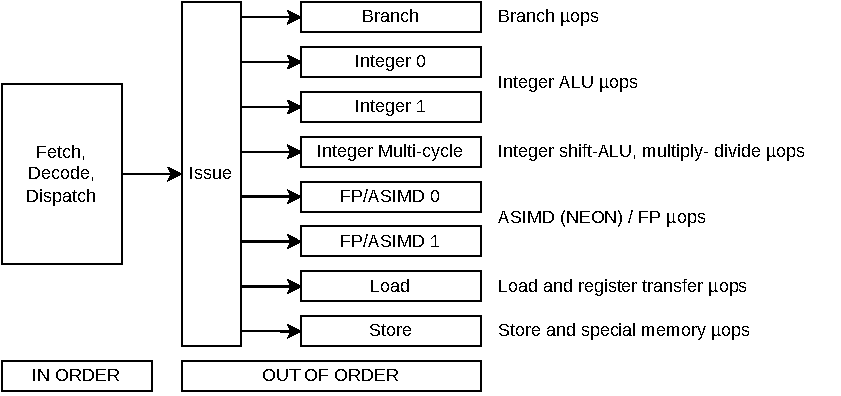
\includegraphics[width=0.7\textwidth]{Figures/a72pipeline.pdf}
    \caption{High-level overview of the Cortex-A72 instruction pipeline}
\end{figure}

The processor might for example store a calculation result, load a necessary
value from memory and execute two SIMD operations at once, all in the same
clock cycle. Modern compilers take advantage of this fact by reordering
instructions such that all pipeline execution units stay as busy as possible
and do not stall while having to wait for new instructions to be dispatched. A
more thorough analysis will be presented for the bitsliced strategy of
\texttt{GIFT}, but all implementations are heavily reliant on function
inlining, instruction reordering and loop unrolling.

\section{GIFT}
\subsection{Table-based}

This is the simplest strategy to implement. Indeed, its biggest advantage lies
in its portability to other platforms without relying on specific features or
extensions. The cipher state is stored as a 64-bit word and one round consists
in extracting the 4-bit S-boxes, looking up table values, collecting these in
an accumulator and finally adding the round key.

% TODO add bitfield extract explanation here

\lstinputlisting[language=c, firstline=77, lastline=87]{../impl/table/gift_table.c}
\lstinputlisting[language=c, firstline=89, lastline=101]{../impl/table/gift_table.c}

\subsection{Using \texttt{vperm}}

Implementation of the substitution layer requires the use of a single vector
intrinsic. This mandates the packing of data into a vector register which in
turn is disadvantageous to the permutation layer as we need to extract single
bits. Packing and unpacking is nothing more than filling 8-bit vector lanes
with 4-bit S-boxes and vice versa.

\lstinputlisting[language=c, firstline=92, lastline=95]{../impl/vector/gift_vec_sbox.c}
\lstinputlisting[language=c, firstline=102, lastline=117]{../impl/vector/gift_vec_sbox.c}
\lstinputlisting[language=c, firstline=197, lastline=212]{../impl/vector/gift_vec_sbox.c}

\subsection{Bitslicing}

We will examine the round function in closer detail and compare the source code
with the generated assembly.
\pagebreak

\begin{lstlisting}[language=c, caption={Round function src}]
for (int round = 0; round < ROUNDS_GIFT_64; round++) {
    gift_64_vec_sliced_subcells(s);
    gift_64_vec_sliced_permute(s);

    // round key addition
    s[0].val[0] = veorq_u8(s[0].val[0], rks[round][0].val[0]);
    s[0].val[1] = veorq_u8(s[0].val[1], rks[round][0].val[1]);
    s[0].val[2] = veorq_u8(s[0].val[2], rks[round][0].val[2]);
    s[0].val[3] = veorq_u8(s[0].val[3], rks[round][0].val[3]);
    s[1].val[0] = veorq_u8(s[1].val[0], rks[round][1].val[0]);
    s[1].val[1] = veorq_u8(s[1].val[1], rks[round][1].val[1]);
    s[1].val[2] = veorq_u8(s[1].val[2], rks[round][1].val[2]);
    s[1].val[3] = veorq_u8(s[1].val[3], rks[round][1].val[3]);
}
\end{lstlisting}

\begin{minipage}{.45\textwidth}
    \begin{lstlisting}[language={[ARM]Assembler}, caption={Round function asm}, escapechar=|]
and     v20.16b, v17.16b, v6.16b
add     x9, x20, x8
eor     v20.16b, v20.16b, v16.16b
add     x8, x8, #0x80|\label{lst:cntrincr}|
and     v21.16b, v20.16b, v19.16b
cmp     x8, #0xe70|\label{lst:cntrchk}|
eor     v21.16b, v21.16b, v6.16b
orr     v6.16b, v6.16b, v16.16b
eor     v6.16b, v6.16b, v17.16b
eor     v16.16b, v19.16b, v6.16b
eor     v17.16b, v16.16b, v20.16b
and     v19.16b, v21.16b, v17.16b
eor     v6.16b, v19.16b, v6.16b
and     v19.16b, v7.16b, v4.16b
eor     v19.16b, v19.16b, v5.16b
and     v20.16b, v19.16b, v18.16b
eor     v20.16b, v20.16b, v4.16b
orr     v4.16b, v4.16b, v5.16b
eor     v4.16b, v4.16b, v7.16b
eor     v5.16b, v18.16b, v4.16b
eor     v7.16b, v5.16b, v19.16b
and     v18.16b, v20.16b, v7.16b
eor     v4.16b, v18.16b, v4.16b
    \end{lstlisting}
\end{minipage}\hfill
\begin{minipage}{.45\textwidth}
    \vspace*{7mm}
    \begin{lstlisting}[language={[ARM]Assembler}, firstnumber=24, escapechar=|]
tbl     v18.16b, {v6.16b}, v2.16b
tbl     v19.16b, {v21.16b}, v3.16b
tbl     v21.16b, {v4.16b}, v2.16b
ldp     q6, q4, [x9, #-112]|\label{lst:floatload}|
mvn     v16.16b, v16.16b
tbl     v16.16b, {v16.16b}, v0.16b
tbl     v17.16b, {v17.16b}, v1.16b
mvn     v5.16b, v5.16b
tbl     v5.16b, {v5.16b}, v0.16b
ldp     q22, q23, [x9, #-80]
eor     v6.16b, v6.16b, v16.16b
eor     v16.16b, v4.16b, v17.16b
tbl     v7.16b, {v7.16b}, v1.16b
eor     v17.16b, v22.16b, v18.16b
tbl     v20.16b, {v20.16b}, v3.16b
ldp     q4, q18, [x9, #-48]
eor     v19.16b, v23.16b, v19.16b
eor     v4.16b, v4.16b, v5.16b
ldp     q22, q23, [x9, #-16]
eor     v5.16b, v18.16b, v7.16b
eor     v7.16b, v22.16b, v21.16b
eor     v18.16b, v23.16b, v20.16b
b.ne    197e0
    \end{lstlisting}
\end{minipage}

Without needing to dive too deep into details, it is obvious to see the
compiler has inlined the two function calls to \texttt{subcells} and
\texttt{permute} with lines 1 to 23 originating from the \texttt{subcells} and
lines 24-46 from the \texttt{permute} and round key addition functions. It has
chosen not to unroll the loop, but has moved the loop counter increment as well
as the condition check in between the \texttt{subcells} instructions to line
\ref{lst:cntrincr} and \ref{lst:cntrchk}. In addition, the loop counter serves
a second purpose as an offset register and is therefore incremented by 0x80=128
instead of just 1.

Permutation (\texttt{tbl}) and round key addition (\texttt{eor}) instructions
are interleaved. The compiler recognizes data dependencies and can therefore
proceed with round key addition immediately after a slice has been permuted
without needing to wait for all permutations to finish. This is only logical
considering the inner workings of the instruction pipeline: by interleaving
NEON with regular logic and load instructions, the execution units are filled
more evenly and pipeline stalls are prevented which speeds up computation.

Round keys are loaded from memory a few instructions before they are needed;
assuming all round keys are stored in the L1 cache, loading a
floating-point/vector register takes 5 cycles. After the load has been
dispatched to the load execution unit in line \ref{lst:floatload}, the
processor happily continues chugging away at the instruction stream by issuing
\texttt{tbl} and \texttt{mvn} $\mu$ops to other execution units.

These kinds of optimizations are pervasive when programming using higher level
languages like C and modern-day compilers more often than not outperform
handcrafted assembly.

\chapter{Evaluation}

In this chapter, we will evaluate the strategies through performance
measurements and discuss advantages, disadvantages and possible use cases.

\section{Benchmarks}

Performance measurements were taken for each strategy as well as for naive
reference implementations and are presented through latency $lat$ in cycles per
byte (c/B) as well as constant throughput $thr$ in MiB/s of the entire
encryption strategy. Round key derivation is measured separately. Measurements
of all individual components like packing or permuting have to be viewed as
upper bounds due to the aforementioned inlining, instruction reordering and
pipelining (TODO REF HERE) taking place in the actual encryption function.

The AArch64 defines system registers in addition to general-purpose registers
which are used for system configuration and monitoring. One of these registers
is the performance monitor cycle count register \texttt{PMCCNTR} which counts
processor clock cycles. Access from userspace is disabled by default and can be
activated through a custom Linux kernel module by setting \texttt{PMUSERENR.EN}
to 1. To minimize interference and because the cycle count register is
core-local, we isolate and utilize one Cortex-A53 and Cortex-A73 core from the
rest of the system for exclusive benchmarking purposes respectively by use of
the \texttt{isolcpus} kernel command line parameter and \texttt{taskset}
command utility.

\subsection{GIFT}

\begin{table}[h!]
    \centering
    \caption{Benchmarks for GIFT}
    \footnotesize
    \begin{tabular}{llcccc}
        \toprule
        & & \multicolumn{2}{c}{Cortex-A53} & \multicolumn{2}{c}{Cortex-A73} \\
        \cmidrule(lr){3-4}\cmidrule(lr){5-6}
        Strategy & Component & $lat$ (c/B) & $thr$ (MiB/s) & $lat$ (c/B) & $thr$ (MiB/s) \\
        \midrule
        \multirow{2}{*}{Naive GIFT-64} & \texttt{round\_keys} & 223.54 & \multirow{2}{*}{1.22} & 190.34 & \multirow{2}{*}{2.33} \\
                                                & \texttt{encrypt} & 1367.66 & &  830.49 & \\
        \cmidrule(lr){2-2}
                                                & \texttt{ subcells} & 4.64 & & 3.13 & \\
                                                & \texttt{  permute} & 36.68 & & 21.09 & \\
        \midrule
        \multirow{2}{*}{Naive GIFT-128} & \texttt{round\_keys} & 182.91 & \multirow{2}{*}{0.51} & 167.16 & \multirow{2}{*}{0.79} \\
                                                 & \texttt{encrypt} & 3532.52 & & 2615.89 & \\
        \cmidrule(lr){2-2}
                                                 & \texttt{ subcells} & 6.91 & & 2.73 & \\
                                                 & \texttt{ permute} & 82.68 & & 61.27 & \\
        \midrule
        \multirow{2}{*}{Table-driven} & \texttt{round\_keys} & 223.81 & \multirow{2}{*}{13.59} & 190.11 & \multirow{2}{*}{16.09} \\
                                      & \texttt{encrypt} & 122.11 & & 119.62 & \\
        \cmidrule(lr){2-2}
                                      & \texttt{ subperm} & 5.15 & & 4.47 & \\
        \midrule
        \multirow{2}{*}{\texttt{vperm} S-box} & \texttt{round\_keys} & 308.12 & \multirow{2}{*}{2.53} & 270.80 & \multirow{2}{*}{3.93} \\
                                              & \texttt{encrypt} & 658.95 & & 492.29 & \\
        \cmidrule(lr){2-2}
                                              & \texttt{ subcells} & 1.63 & & 1.13 & \\
                                              & \texttt{ permute} & 22.71 & & 15.24 & \\
                                              & \texttt{ pack} & 7.51 & & 2.94 & \\
                                              & \texttt{ unpack} & 8.76 & & 5.89 & \\
        \midrule
        \multirow{2}{*}{Bitsliced} & \texttt{round\_keys} & 10.13 & \multirow{2}{*}{111.89} & 7.66 & \multirow{2}{*}{154.21} \\
                                   & \texttt{encrypt} & 16.22 & & 13.51 & \\
        \cmidrule(lr){2-2}
                                   & \texttt{ subcells} & 0.41 & & 0.18 & \\
                                   & \texttt{ permute} & 0.39 & & 0.09 & \\
                                   & \texttt{ pack} & 1.48 & & 1.01 & \\
                                   & \texttt{ unpack} & 1.49 & & 1.01 & \\
        \bottomrule
    \end{tabular}
\end{table}

\subsection{Camellia}

\begin{table}[h!]
    \centering
    \caption{Benchmarks for Camellia}
    \scriptsize
    \begin{tabular}{llcccc}
        \toprule
        & & \multicolumn{2}{c}{Cortex-A53} & \multicolumn{2}{c}{Cortex-A73} \\
        \cmidrule(lr){3-4}\cmidrule(lr){5-6}
        Strategy & Component & $lat$ (c/B) & $thr$ (MiB/s) & $lat$ (c/B) & $thr$ (MiB/s) \\
        \midrule
        \multirow{2}{*}{Naive Camellia-128} & \texttt{round\_keys} & 15.26 & \multirow{2}{*}{33.74} & 11.08 & \multirow{2}{*}{46.71} \\
                                                & \texttt{encrypt} & 53.44 & &  43.51 & \\
        \cmidrule(lr){2-2}
                                                & \texttt{ feistel\_round} & 4.02 & & 2.66 & \\
                                                & \texttt{ S} & 2.01 & & 0.94 & \\
                                                & \texttt{ F} & 3.13 & & 2.25 & \\
                                                & \texttt{ P} & 2.03 & & 1.63 & \\
                                                & \texttt{ FL} & 1.06 & & 0.72 & \\
        \midrule
        \multirow{2}{*}{Naive Camellia-256} & \texttt{round\_keys} & 22.01 & \multirow{2}{*}{25.50} & 16.99 & \multirow{2}{*}{35.16} \\
                                                 & \texttt{encrypt} & 70.55 & & 58.27 & \\
        \midrule
        \multirow{2}{*}{Optimized Camellia-128} & \texttt{round\_keys} & 8.18 & \multirow{2}{*}{77.07} & 5.93 & \multirow{2}{*}{107.31} \\
                                                & \texttt{encrypt} & 23.63 & & 19.83 & \\
        \cmidrule(lr){2-2}
                                                & \texttt{ feistel\_round} & 2.32 & & 1.56 & \\
                                                & \texttt{ F} & 2.21 & & 1.43 & \\
                                                & \texttt{ FL} & 1.06 & & 0.69 & \\
        \midrule
        \multirow{2}{*}{Byte-sliced Camellia-128} & \texttt{round\_keys} & 2.59 & \multirow{2}{*}{106.20} & 2.19 & \multirow{2}{*}{138.42} \\
                                                & \texttt{encrypt} & 17.14 & & 15.11 & \\
        \cmidrule(lr){2-2}
                                                & \texttt{ feistel\_round} & 1.00 & & 0.69 & \\
                                                & \texttt{ F} & 0.79 & & 0.58 & \\
                                                & \texttt{ FL} & 0.36 & & 0.13 & \\
                                                & \texttt{ pack} & 1.04 & & 0.96 & \\
                                                & \texttt{ unpack} & 0.91 & & 0.83 & \\
        \bottomrule
    \end{tabular}
\end{table}

\chapter*{Acknowledgements}

I want to thank ...

\appendix
\chapter{Detailed benchmarking results}
\label{app:benchmarks}

\section{GIFT}

\begin{table}[!htbp]
    \centering
    \caption{Benchmarks for GIFT}
    \scriptsize
    \begin{tabular}{llcccc}
        \toprule
        & & \multicolumn{2}{c}{Cortex-A53} & \multicolumn{2}{c}{Cortex-A73} \\
        \cmidrule(lr){3-4}\cmidrule(lr){5-6}
        Strategy & Component & $lat$ (c/B) & $thr$ (MiB/s) & $lat$ (c/B) & $thr$ (MiB/s) \\
        \midrule
        \multirow{2}{*}{Naive GIFT-64} & \texttt{round\_keys} & 223.54 & \multirow{2}{*}{1.22} & 190.34 & \multirow{2}{*}{2.33} \\
                                                & \texttt{encrypt} & 1367.66 & &  830.49 & \\
        \cmidrule(lr){2-2}
                                                & \texttt{ subcells} & 4.64 & & 3.13 & \\
                                                & \texttt{  permute} & 36.68 & & 21.09 & \\
        \midrule
        \multirow{2}{*}{Naive GIFT-128} & \texttt{round\_keys} & 182.91 & \multirow{2}{*}{0.51} & 167.16 & \multirow{2}{*}{0.79} \\
                                                 & \texttt{encrypt} & 3532.52 & & 2615.89 & \\
        \cmidrule(lr){2-2}
                                                 & \texttt{ subcells} & 6.91 & & 2.73 & \\
                                                 & \texttt{ permute} & 82.68 & & 61.27 & \\
        \midrule
        \multirow{2}{*}{Table-driven} & \texttt{round\_keys} & 223.81 & \multirow{2}{*}{13.59} & 190.11 & \multirow{2}{*}{16.09} \\
                                      & \texttt{encrypt} & 122.11 & & 119.62 & \\
        \cmidrule(lr){2-2}
                                      & \texttt{ subperm} & 5.15 & & 4.47 & \\
        \midrule
        \multirow{2}{*}{\texttt{vperm} S-box} & \texttt{round\_keys} & 308.12 & \multirow{2}{*}{1.10} & 270.69 & \multirow{2}{*}{1.58} \\
                                              & \texttt{encrypt} & 1514.28 & & 1218.18 & \\
        \cmidrule(lr){2-2}
                                              & \texttt{ subcells} & 1.63 & & 1.13 & \\
                                              & \texttt{ permute} & 53.18 & & 42.40 & \\
                                              & \texttt{ pack} & 7.51 & & 1.24 & \\
                                              & \texttt{ unpack} & 7.39 & & 4.67 & \\
        \midrule
        \multirow{2}{*}{Bitsliced} & \texttt{round\_keys} & 19.93 & \multirow{2}{*}{108.80} & 16.12 & \multirow{2}{*}{150.50} \\
                                   & \texttt{encrypt} & 16.69 & & 13.98 & \\
        \cmidrule(lr){2-2}
                                   & \texttt{ subcells} & 0.41 & & 0.06 & \\
                                   & \texttt{ permute} & 0.39 & & 0.18 & \\
                                   & \texttt{ pack} & 1.81 & & 1.34 & \\
                                   & \texttt{ unpack} & 1.68 & & 1.31 & \\
        \bottomrule
    \end{tabular}
\end{table}

\section{Camellia}

\begin{table}[!htpb]
    \centering
    \caption{Benchmarks for Camellia}
    \scriptsize
    \begin{tabular}{llcccc}
        \toprule
        & & \multicolumn{2}{c}{Cortex-A53} & \multicolumn{2}{c}{Cortex-A73} \\
        \cmidrule(lr){3-4}\cmidrule(lr){5-6}
        Strategy & Component & $lat$ (c/B) & $thr$ (MiB/s) & $lat$ (c/B) & $thr$ (MiB/s) \\
        \midrule
        \multirow{2}{*}{Naive Camellia-128} & \texttt{round\_keys} & 15.26 & \multirow{2}{*}{33.74} & 11.08 & \multirow{2}{*}{46.71} \\
                                                & \texttt{encrypt} & 53.44 & &  43.51 & \\
        \cmidrule(lr){2-2}
                                                & \texttt{ feistel\_round} & 4.02 & & 2.66 & \\
                                                & \texttt{ S} & 2.01 & & 0.94 & \\
                                                & \texttt{ F} & 3.13 & & 2.25 & \\
                                                & \texttt{ P} & 2.03 & & 1.63 & \\
                                                & \texttt{ FL} & 1.06 & & 0.72 & \\
        \midrule
        \multirow{2}{*}{Naive Camellia-256} & \texttt{round\_keys} & 22.01 & \multirow{2}{*}{25.50} & 16.99 & \multirow{2}{*}{35.16} \\
                                                 & \texttt{encrypt} & 70.55 & & 58.27 & \\
        \midrule
        \multirow{2}{*}{Optimized Camellia-128} & \texttt{round\_keys} & 8.18 & \multirow{2}{*}{77.07} & 5.93 & \multirow{2}{*}{107.31} \\
                                                & \texttt{encrypt} & 23.63 & & 19.83 & \\
        \cmidrule(lr){2-2}
                                                & \texttt{ feistel\_round} & 2.32 & & 1.56 & \\
                                                & \texttt{ F} & 2.21 & & 1.43 & \\
                                                & \texttt{ FL} & 1.06 & & 0.69 & \\
        \midrule
        \multirow{2}{*}{Bytesliced Camellia-128} & \texttt{round\_keys} & 2.59 & \multirow{2}{*}{106.20} & 2.19 & \multirow{2}{*}{138.42} \\
                                                & \texttt{encrypt} & 17.14 & & 15.19 & \\
        \cmidrule(lr){2-2}
                                                & \texttt{ feistel\_round} & 1.00 & & 0.69 & \\
                                                & \texttt{ F} & 0.79 & & 0.58 & \\
                                                & \texttt{ FL} & 0.36 & & 0.12 & \\
                                                & \texttt{ pack} & 1.04 & & 0.96 & \\
                                                & \texttt{ unpack} & 0.91 & & 0.83 & \\
        \bottomrule
    \end{tabular}
\end{table}

\chapter{List of symbols}

\begin{center}
    \begin{tabular}{rl}
        $\ll_n/\gg_n$ & left/right shift by $n$ bits \\
        $\lll_n/\ggg_n$ & left/right rotate by $n$ bits \\
        $\land$ & AND \\
        $\lor$ & OR \\
        $\lnot$ & NOT \\
        $\oplus$ & XOR \\
        $A_{(32)}$ & $A$ is 32 bits long \\
        $A_{21}\leftarrow 1$ & set bit $21$ of $A$ to $1$ \\
        $||$ & concatenation
    \end{tabular}
\end{center}

\chapter{C source code}
\label{app:cimpl}

\section{GIFT}
\subsection{Table-based}

\lstinputlisting[language=c, caption={\texttt{gift/table.h}}]{../impl/gift/table.h}
\lstinputlisting[language=c, caption={\texttt{gift/table.c}}]{../impl/gift/table.c}

\subsection{Using \texttt{vperm}}

\lstinputlisting[language=c, caption={\texttt{gift/vec\_sbox.h}}]{../impl/gift/vec_sbox.h}
\lstinputlisting[language=c, caption={\texttt{gift/vec\_sbox.c}}]{../impl/gift/vec_sbox.c}

\subsection{Bitslicing}

\lstinputlisting[language=c, caption={\texttt{gift/vec\_sliced.h}}]{../impl/gift/vec_sliced.h}
\lstinputlisting[language=c, caption={\texttt{gift/vec\_sliced.c}}]{../impl/gift/vec_sliced.c}

\section{Camellia}

\subsection{Optimized non-SIMD}

\lstinputlisting[language=c, caption={\texttt{camellia/spec\_opt.h}}]{../impl/camellia/spec_opt.h}
\lstinputlisting[language=c, caption={\texttt{camellia/spec\_opt.c}}]{../impl/camellia/spec_opt.c}

\subsection{Byteslicing}

\lstinputlisting[language=c, caption={\texttt{camellia/bytesliced.h}}]{../impl/camellia/bytesliced.h}
\lstinputlisting[language=c, caption={\texttt{camellia/bytesliced.c}}]{../impl/camellia/bytesliced.c}


\printbibliography

\end{document}
